\documentclass{beamer}
\usepackage[utf8]{inputenc}

\usetheme{Madrid}
\usecolortheme{default}
\usepackage{amsmath,amssymb,amsfonts,amsthm}
\usepackage{txfonts}
\usepackage{tkz-euclide}
\usepackage{listings}
\usepackage{adjustbox}
\usepackage{array}
\usepackage{tabularx}
\usepackage{gvv}
\usepackage{lmodern}
\usepackage{circuitikz}
\usepackage{tikz}
\usepackage{graphicx}
\usepackage{mathtools}
\setbeamertemplate{page number in head/foot}[totalframenumber]

\usepackage{tcolorbox}
\tcbuselibrary{minted,breakable,xparse,skins}



\definecolor{bg}{gray}{0.95}
\DeclareTCBListing{mintedbox}{O{}m!O{}}{%
  breakable=true,
  listing engine=minted,
  listing only,
  minted language=#2,
  minted style=default,
  minted options={%
    linenos,
    gobble=0,
    breaklines=true,
    breakafter=,,
    fontsize=\small,
    numbersep=8pt,
    #1},
  boxsep=0pt,
  left skip=0pt,
  right skip=0pt,
  left=25pt,
  right=0pt,
  top=3pt,
  bottom=3pt,
  arc=5pt,
  leftrule=0pt,
  rightrule=0pt,
  bottomrule=2pt,
  toprule=2pt,
  colback=bg,
  colframe=orange!70,
  enhanced,
  overlay={%
    \begin{tcbclipinterior}
    \fill[orange!20!white] (frame.south west) rectangle ([xshift=20pt]frame.north west);
    \end{tcbclipinterior}},
  #3,
}
\lstset{
    language=C,
    basicstyle=\ttfamily\small,
    keywordstyle=\color{blue},
    stringstyle=\color{orange},
    commentstyle=\color{green!60!black},
    numbers=left,
    numberstyle=\tiny\color{gray},
    breaklines=true,
    showstringspaces=false,
}
%This block of code defines the information to appear in the
%Title page
\title %optional
{4.7.56}
%\subtitle{A short story}

\author % (optional)
{Vaishnavi - EE25BTECH11059}



\begin{document}


\frame{\titlepage}
\begin{frame}{Question}
Find the equation of the line whose perpendicular distance from the origin is $4$ units and the angle which the normal makes with positive direction of x-axis is $15^\circ$
\end{frame}
\begin{frame}{allowframebreaks}
\frametitle{Solution}
\begin{table}[H]    
  \centering
  \begin{tabular}{|c|c|}
\hline
\textbf{Variable} & \textbf{Value} \\
\hline
$A$ & $(0,-\frac{3}{2})$ \\
\hline
$m$ & $\frac{1}{2}$ \\
\hline
\end{tabular}
  \caption{Variables Used}
  \label{tab:1.10.2}
\end{table}

\end{frame}


\begin{frame}{Solution}
Let eq of line be
\begin{align}
\vec{n^T}\vec{x}=c
\end{align}
where,
\begin{align}
\vec{n}=\myvec{cos 15^\circ
               \\
               sin 15^\circ}
\end{align}
eq of line is
\begin{align}
\myvec{cos 15^\circ & sin 15^\circ}
\vec{x}
=c
\end{align}
\end{frame}

\begin{frame}{solution}
As distance from origin (d)=$4$ units
\begin{align}
    \frac{|c|}{\|n\|}=4\\
    \frac{|c|}{1}=4\\
    c=\pm 4
\end{align}   


Hence eq of line is 
\begin{align}
\myvec{cos 15^\circ & sin 15^\circ}
\vec{x}
=\pm4
\end{align}

\end{frame}
\begin{frame}{Graph}
   Refer to Figure

\begin{figure}[H]
\begin{center}
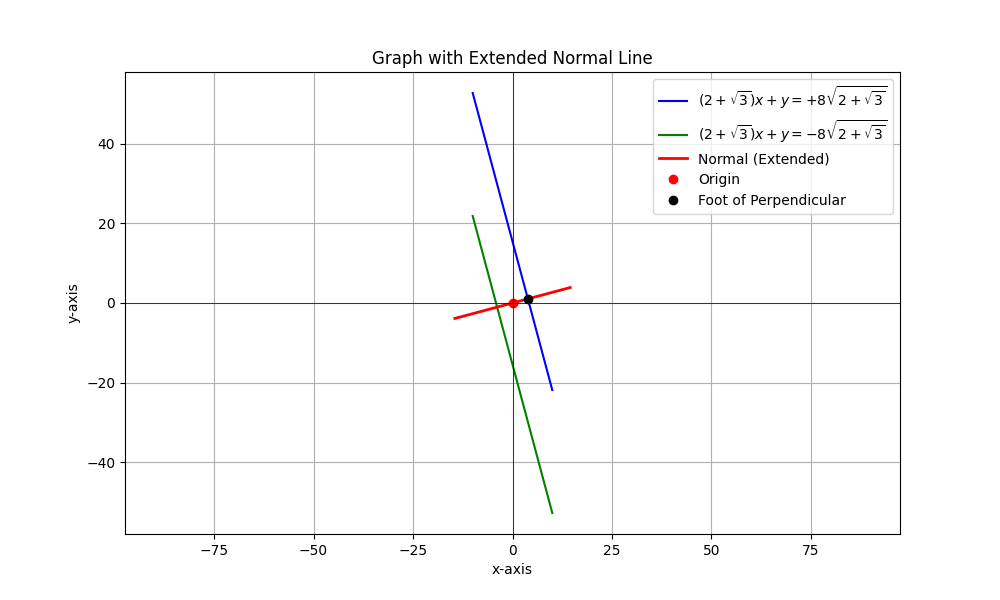
\includegraphics[width=0.6\columnwidth]{../figs/graph7.png}
\end{center}
\caption{}
\label{fig:Fig}
\end{figure}  
\end{frame}




\begin{frame}[fragile]
    \frametitle{Python Code}
    \begin{lstlisting}
import matplotlib.pyplot as plt
import numpy as np

# Constants
sqrt3 = np.sqrt(3)
A = 2 + sqrt3
B = 1
C = 8 * np.sqrt(2 + sqrt3)

# Create x values
x = np.linspace(-10, 10, 400)

# Two lines: one for +C and one for -C
y1 = -A * x + C  # Line 1
y2 = -A * x - C  # Line 2

# Plotting
plt.figure(figsize=(10, 6))
plt.plot(x, y1, label=r'$(2+\sqrt{3})x + y = +8\sqrt{2+\sqrt{3}}$', color='blue')
plt.plot(x, y2, label=r'$(2+\sqrt{3})x + y = -8\sqrt{2+\sqrt{3}}$', color='green')

\end{lstlisting}
\end{frame}

\begin{frame}[fragile]
    \frametitle{Python Code }

    \begin{lstlisting}
# === Calculate the foot of the perpendicular from origin to line1 ===
x0, y0 = 0, 0
A_val = A
B_val = 1
C_val = -C  # Rewrite as Ax + By + C = 0

denominator = A_val**2 + B_val**2
x_foot = (B_val * (B_val * x0 - A_val * y0) - A_val * C_val) / denominator
y_foot = (A_val * (A_val * y0 - B_val * x0) - B_val * C_val) / denominator

# === Draw extended solid normal line through origin and foot ===
# Direction vector of normal = (A, B)


    \end{lstlisting}
\end{frame}

\begin{frame}[fragile]
    \frametitle{Python Code}

    \begin{lstlisting}
normal_length = 15  # increase to make longer
unit_normal = np.array([A_val, B_val]) / np.sqrt(denominator)
start_point = -normal_length * unit_normal
end_point = normal_length * unit_normal

plt.plot([start_point[0], end_point[0]], [start_point[1], end_point[1]],
         color='red', linewidth=2, label='Normal (Extended)')

# Plot origin and foot point
plt.plot(0, 0, 'ro', label='Origin')
plt.plot(x_foot, y_foot, 'ko', label='Foot of Perpendicular')

# Axes
plt.axhline(0, color='black', linewidth=0.5)
plt.axvline(0, color='black', linewidth=0.5)



  \end{lstlisting}
\end{frame}
\begin{frame}[fragile]
    \frametitle{Python Code}

    \begin{lstlisting}
# Formatting
plt.title('Graph with Extended Normal Line')
plt.xlabel('x-axis')
plt.ylabel('y-axis')
plt.grid(True)
plt.axis('equal')
plt.legend()

# Save and show plot
plt.savefig("graph7_with_extended_normal.png")
plt.show()



  \end{lstlisting}
\end{frame}
\begin{frame}[fragile]
\frametitle{C Code}
\begin{lstlisting}
#include <stdio.h>
#include <math.h>

// Function to compute normal vector, magnitude, and constants
void compute_line_params(double m, double d, double* A, double* B, double* C1, double* C2) {
    // Normal vector n = (-m, 1)
    *A = -m;
    *B = 1.0;

    // Norm of the vector
    double norm = sqrt((*A) * (*A) + (*B) * (*B));

    // |c| = d * ||n||
    double abs_c = d * norm;

    // ±c values
    *C1 = abs_c;
    *C2 = -abs_c;
}

    \end{lstlisting}

\end{frame}

\begin{frame}[fragile]
\frametitle{C Code}
\begin{lstlisting}
 int main() {
    double m = -2.0 - sqrt(3.0);  // Given slope
    double d = 4.0;               // Perpendicular distance from origin

    double A, B, C1, C2;

    // Compute parameters
    compute_line_params(m, d, &A, &B, &C1, &C2);

    // Display the results
    printf("Equation of the lines:\n");
    printf("%.4fx + %.4fy = %.4f\n", A, B, C1);
    printf("%.4fx + %.4fy = %.4f\n", A, B, C2);

    return 0;
}

\end{lstlisting}
\end{frame}

\begin{frame}[fragile]
\frametitle{Python and C Code}

\begin{lstlisting}
import ctypes
from ctypes import c_double, POINTER

# Load the compiled shared object
lib = ctypes.CDLL("./code.so")

# Define argument and return types for the function
lib.compute_line_params.argtypes = [c_double, c_double,
                                    POINTER(c_double), POINTER(c_double),
                                    POINTER(c_double), POINTER(c_double)]

# Inputs
m = -2 - 3**0.5  # given slope
d = 4.0          # distance from origin

\end{lstlisting}

\end{frame}
\begin{frame}[fragile]
\frametitle{Python and C Code}

\begin{lstlisting}
# Outputs
A = c_double()
B = c_double()
C1 = c_double()
C2 = c_double()

# Call the C function
lib.compute_line_params(m, d, ctypes.byref(A), ctypes.byref(B), ctypes.byref(C1), ctypes.byref(C2))

# Print the result
print("Equation of the line(s):")
print(f"{A.value:.4f}x + {B.value:.4f}y = {C1.value:.4f}")
print(f"{A.value:.4f}x + {B.value:.4f}y = {C2.value:.4f}")


\end{lstlisting}

\end{frame}
\end{document}